\chapter{Banco de registradores (\texttt{reg\_bank})}
\label{cap:reg_bank}

\section{Especificação}

O \texttt{reg\_bank} é um banco de quatro registradores de 8 bits, chamados R0 a R3 \cite{tp2}. A \textbf{leitura} é feita por duas saídas simultâneas, \texttt{a\_do} e \texttt{b\_do}, cada uma com sua entrada de seleção (\texttt{a\_sel} e \texttt{b\_sel}); ela é assíncrona (independe do clock) e não tem habilitação. A \textbf{escrita} é síncrona, na borda de subida de \texttt{clk\_in}, e só ocorre com \texttt{wr\_ena} em nível alto; o registrador escrito é o apontado por \texttt{a\_sel}, e o dado vem de \texttt{di}. O reset assíncrono (\texttt{nrst}, ativo em nível baixo) zera os quatro registradores e tem preferência sobre todas as outras entradas. A Figura~\ref{fig:bloco-reg-bank} mostra o diagrama de blocos e o Quadro~\ref{quad:portas-reg-bank} descreve as portas.

\begin{figure}[htb]
\caption{Diagrama de blocos do banco de registradores.}\label{fig:bloco-reg-bank}
\centering
\begin{tikzpicture}[>={Stealth[length=2mm]}]
  \node[draw, minimum width=3.2cm, minimum height=5.2cm, font=\large\bfseries] (bloco) {reg\_bank};
  \pentrada{2.1}{nrst}{}
  \pentrada{1.3}{clk\_in}{}
  \pentrada{0.5}{di[7..0]}{line width=1.2pt}
  \pentrada{-0.3}{a\_sel[1..0]}{line width=1.2pt}
  \pentrada{-1.1}{b\_sel[1..0]}{line width=1.2pt}
  \pentrada{-1.9}{wr\_ena}{}
  \psaida{0.8}{a\_do[7..0]}{line width=1.2pt}
  \psaida{-0.8}{b\_do[7..0]}{line width=1.2pt}
\end{tikzpicture}
\fonte{Elaborada pelos autores, com base em \textcite{tp2}.}
\end{figure}

\begin{quadro}[htb]
  \caption{Portas do banco de registradores.}
  \label{quad:portas-reg-bank}
  \centering
  \begin{tabular}{lcp{9cm}}
    \hline
    Porta & Direção & Descrição \\ \hline
    \texttt{nrst} & entrada & \textit{Reset} assíncrono, ativo em nível baixo; zera R0 a R3 e vence todas as outras entradas \\
    \texttt{clk\_in} & entrada & Clock; a escrita acontece na borda de subida \\
    \texttt{di[7..0]} & entrada & Dado a ser escrito \\
    \texttt{a\_sel[1..0]} & entrada & Seleciona o registrador lido em \texttt{a\_do} e o escrito, quando \texttt{wr\_ena = '1'} \\
    \texttt{b\_sel[1..0]} & entrada & Seleciona o registrador lido em \texttt{b\_do} \\
    \texttt{wr\_ena} & entrada & Habilitação de escrita, ativa em nível alto \\
    \texttt{a\_do[7..0]} & saída & Conteúdo do registrador selecionado por \texttt{a\_sel} (combinacional) \\
    \texttt{b\_do[7..0]} & saída & Conteúdo do registrador selecionado por \texttt{b\_sel} (combinacional) \\ \hline
  \end{tabular}
  \fonte{Adaptado de \textcite{tp2}.}
\end{quadro}

O texto da especificação chama a habilitação de escrita de \texttt{wr\_ena} e o diagrama a chama de \texttt{wr\_en}; adotou-se \texttt{wr\_ena}, que é o nome usado na descrição das entradas.

\section{Implementação}

\subsection{Arquitetura}

Os quatro registradores formam um único sinal, um \textit{array} de quatro vetores de 8 bits (\texttt{r(0)} é R0, e assim por diante). As seleções \texttt{a\_sel} e \texttt{b\_sel} são convertidas em inteiros de 0 a 3 e usadas como índices do \textit{array}. O código tem duas partes:

\begin{itemize}
  \item \textbf{Leitura}: duas atribuições concorrentes, \texttt{a\_do <= r(a\_idx)} e \texttt{b\_do <= r(b\_idx)}. Como estão fora de qualquer processo, as saídas reagem à seleção e ao conteúdo dos registradores sem esperar o clock, e como as duas atribuições são independentes, as duas leituras podem apontar para registradores diferentes ou para o mesmo.
  \item \textbf{Escrita}: um \texttt{process} sensível a \texttt{nrst} e \texttt{clk\_in}. O teste de \texttt{nrst = '0'} vem primeiro e zera todo o \textit{array} com um agregado; só então vem o \texttt{ELSIF RISING\_EDGE(clk\_in)}, e dentro dele a escrita \texttt{r(a\_idx) <= di} só ocorre se \texttt{wr\_ena = '1'}. Sem \texttt{wr\_ena} nada é atribuído, e os registradores mantêm o valor.
\end{itemize}

\subsection{Decisões de projeto}

\begin{itemize}
  \item \textbf{\textit{Array} em vez de quatro sinais}: o decodificador de escrita e os multiplexadores de leitura do diagrama funcional da especificação são gerados pelo sintetizador a partir do índice, o que evita repetir o mesmo código quatro vezes.
  \item \textbf{Faixa do índice}: os sinais \texttt{a\_idx} e \texttt{b\_idx} são declarados \texttt{INTEGER RANGE 0 TO 3}, de modo que o sintetizador usa apenas 2 bits e o índice nunca sai do \textit{array}.
  \item \textbf{Leitura durante a escrita}: quando \texttt{a\_sel} aponta para o registrador que está sendo escrito, \texttt{a\_do} mostra o valor \textit{antigo} até a borda de subida e o novo logo depois dela, porque a saída lê o registrador, e não a entrada \texttt{di}.
\end{itemize}

\subsection{Circuito em nível RTL}

A Figura~\ref{fig:rtl-reg-bank} mostra a interpretação do código feita pela ferramenta RapidRTL. Aparecem quatro registradores de 8 bits com reset assíncrono e habilitação (\texttt{\$adffe}), a lógica que decodifica \texttt{a\_sel} e \texttt{wr\_ena} nas quatro habilitações (portas E e inversores) e dois multiplexadores 4:1 (\texttt{\$bmux}) que levam o conteúdo dos registradores às saídas \texttt{a\_do} e \texttt{b\_do}. É, portanto, a mesma estrutura do diagrama funcional da especificação.

\begin{figure}[htb]
  \centering
  \caption{Circuito do banco de registradores em nível RTL.}
  \label{fig:rtl-reg-bank}
  \includegraphics[width=\textwidth, height=0.6\textheight, keepaspectratio]{reg_bank_rtl.pdf}
  \fonte{Elaborado a partir do site RapidRTL, com base no arquivo \texttt{project/reg\_bank/reg\_bank.vhd}.}
\end{figure}

\subsection{Código-fonte}

O Código~\ref{lst:reg-bank} apresenta a entidade e a arquitetura completas, com comentários.

\blocovhdl{Descrição VHDL do banco de registradores.}{lst:reg-bank}{reg_bank}{reg_bank.vhd}

\section{Simulação e resultados}

\subsection{Metodologia}

O projeto tem cinco formas de onda (arquivos \texttt{.vwf} em \texttt{project/reg\_bank/}), todas com clock de 20\,ns e reset inicial:

\begin{itemize}
  \item \texttt{reg\_bank.vwf}: visão geral, com escrita nos quatro registradores, leitura simultânea, escrita bloqueada, reset assíncrono e nova escrita;
  \item \texttt{reg\_bank\_escrita.vwf}: escrita de cada registrador, com releitura pela porta B, e sobrescrita;
  \item \texttt{reg\_bank\_leitura.vwf}: varredura das 16 combinações de (\texttt{a\_sel}, \texttt{b\_sel}), com os seletores mudando 5\,ns antes da borda, para mostrar que a leitura é assíncrona;
  \item \texttt{reg\_bank\_wr\_ena.vwf}: efeito de \texttt{wr\_ena} sem escrita, com um pulso entre bordas (que não escreve) e um pulso sobre a borda de subida (que escreve);
  \item \texttt{reg\_bank\_reset.vwf}: reset fora de qualquer borda, reset prevalecendo sobre a escrita e pulso curto de reset.
\end{itemize}

Além delas, o \textit{testbench} \texttt{extras/reg\_bank\_tb.vhd} compara as 16 combinações de leitura com um modelo de referência a cada ciclo, em casos direcionados e em 400 ciclos pseudoaleatórios. Ele executa 6\,608 comparações, sem nenhuma falha. As tabelas de resultados esperados de todas as formas de onda estão em \texttt{extras/casos\_de\_teste.md}.

\subsection{Casos de teste e resultados}

A Figura~\ref{fig:sim-reg-bank} mostra a simulação de \texttt{reg\_bank.vwf} e a Tabela~\ref{tab:caso-reg-bank} traz os valores esperados. Cada linha da tabela é um intervalo entre mudanças das entradas, e as saídas mostradas são as do fim do intervalo, depois de qualquer borda de subida dentro dele. As tabelas das demais formas de onda estão no Apêndice~\ref{ap:tabelas}.

\begin{figure}[htb]
  \centering
  \caption{Simulação funcional de \texttt{reg\_bank.vwf} (visão geral).}
  \label{fig:sim-reg-bank}
  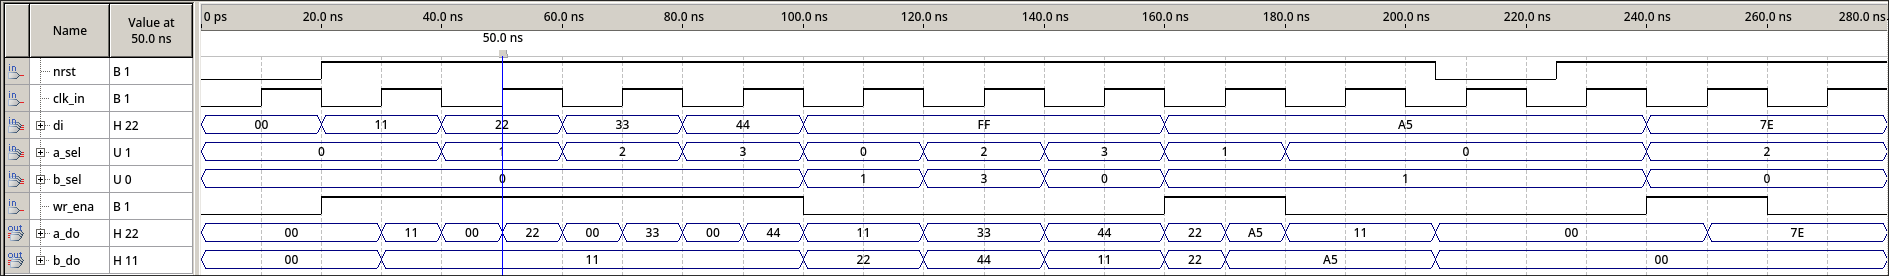
\includegraphics[width=\textwidth]{../../project/reg_bank/reg_bank_simulation.png}
  \fonte{Autoria própria (Quartus II).}
\end{figure}

\Needspace*{12\baselineskip}
{\scriptsize\setlength{\tabcolsep}{3pt}
\begin{longtable}{rcccccccp{5.3cm}}
\caption{Casos de teste de \texttt{reg\_bank.vwf}: visão geral.}
\label{tab:caso-reg-bank}\\
\hline $t$ (ns) & \texttt{nrst} & \texttt{di} & \texttt{a\_sel} & \texttt{b\_sel} & \texttt{wr\_ena} & \texttt{a\_do} & \texttt{b\_do} & Observação \\ \hline \endfirsthead
\hline $t$ (ns) & \texttt{nrst} & \texttt{di} & \texttt{a\_sel} & \texttt{b\_sel} & \texttt{wr\_ena} & \texttt{a\_do} & \texttt{b\_do} & Observação \\ \hline \endhead
0--20 & 0 & 00h & 0 & 0 & 0 & 00h & 00h &  \\
20--40 & 1 & 11h & 0 & 0 & 1 & 11h & 11h & solta o reset; escreve 11h em R0 \\
40--60 & 1 & 22h & 1 & 0 & 1 & 22h & 11h & escreve 22h em R1 \\
60--80 & 1 & 33h & 2 & 0 & 1 & 33h & 11h & escreve 33h em R2 \\
80--100 & 1 & 44h & 3 & 0 & 1 & 44h & 11h & escreve 44h em R3 \\
100--120 & 1 & FFh & 0 & 1 & 0 & 11h & 22h & wr\_ena = 0: lê R0 e R1 (di = FFh é ignorado) \\
120--140 & 1 & FFh & 2 & 3 & 0 & 33h & 44h & lê R2 e R3 \\
140--160 & 1 & FFh & 3 & 0 & 0 & 44h & 11h & lê R3 e R0 \\
160--180 & 1 & A5h & 1 & 1 & 1 & A5h & A5h & escreve A5h em R1 (a\_sel = b\_sel = 1) \\
180--205 & 1 & A5h & 0 & 1 & 0 & 11h & A5h & lê R0 e R1 \\
205--225 & 0 & A5h & 0 & 1 & 0 & 00h & 00h & reset assíncrono no meio do ciclo (nrst = 0) \\
225--240 & 1 & A5h & 0 & 1 & 0 & 00h & 00h & solta o reset \\
240--260 & 1 & 7Eh & 2 & 0 & 1 & 7Eh & 00h & escreve 7Eh em R2 \\
260--280 & 1 & 7Eh & 2 & 0 & 0 & 7Eh & 00h & lê R2 e R0 \\
\hline
\end{longtable}}
\vspace{-0.9cm}
\fonte{Autoria própria. Saídas do fim de cada intervalo, conforme o modelo de referência e a simulação do Quartus II.}


\subsection{Análise dos resultados}

Os resultados confirmam o comportamento especificado:

\begin{itemize}
  \item \textbf{Escrita}: R0, R1, R2 e R3 recebem 11h, 22h, 33h e 44h nas bordas de subida em 30, 50, 70 e 90\,ns. A escrita só aparece na saída \textit{depois} da borda: no intervalo 40--60\,ns, por exemplo, \texttt{a\_do} mostra 00h (valor antigo de R1) até a borda em 50\,ns e 22h em seguida.
  \item \textbf{Leitura de dois registradores}: de 100 a 160\,ns, \texttt{a\_do} e \texttt{b\_do} mostram registradores diferentes ao mesmo tempo (R0 e R1, R2 e R3, R3 e R0), sem escrita e sem relação com o valor de \texttt{di}, que fica em FFh.
  \item \textbf{\texttt{wr\_ena}}: com \texttt{wr\_ena = '0'} nenhum registrador muda, mesmo com bordas de clock e \texttt{di} diferente de zero. Quando \texttt{a\_sel = b\_sel = 1} e \texttt{wr\_ena = '1'}, as duas saídas mostram A5h depois da borda.
  \item \textbf{Reset assíncrono}: em 205\,ns, no meio do ciclo, \texttt{nrst} cai e as duas saídas vão a 00h na hora, sem esperar a borda seguinte; o reset segue ativo durante a borda de 210\,ns. Depois que é solto, a escrita de 7Eh em R2 volta a funcionar.
\end{itemize}

Nas formas de onda \texttt{reg\_bank\_wr\_ena.vwf} e \texttt{reg\_bank\_reset.vwf} aparecem os casos que dependem de a memória ser mesmo um \textit{flip-flop} disparado por borda: o pulso de \texttt{wr\_ena} entre duas bordas não escreve (um \textit{latch} escreveria), e o reset vence a escrita quando as duas coincidem em uma borda de subida.
